\chapter{Electrical Quantities \& Components}

\section{Electrical quantities}

\subsection{Electric charges}\index{charge}

Electric charge is the property of matter that causes it to experience a force in an electric field.  Electric charges come in two types, \emph{positive} charges (+ve) and \emph{negative} charges (-ve) \footnote{Important to realise that the +ve and -ve signs are to distinguish each type. A -ve charge is not an deficit of charge in the way that a -ve bank account is a debt.}. You should be familiar with the fact that like charges repel each other, and opposite charges attract. The interaction between electric charges plays a central role in all electrostatic, chemical and electrical phenomena.

Electric charges are measured in coulombs: $[Q] = \text{C}$\\

All matter is made of atoms, which consist of a nucleus (+ve) and electrons (-ve) and each electron has a charge of $-e$, where $e=1.60\times10^{-19}\text{ C}$ is the \keypoint{elementary charge}.

Typically a body becomes electrically-charged by losing or gaining electrons.

\begin{itemize}
	\item[--] an object that gains electrons from elsewhere becomes negatively-charged
	
	\item[--] an object that loses electrons becomes positively-charged
\end{itemize}


The charge of any object must be an integer multiple of the elementary charge: $\tcbhighmath{Q=Ne}$ This is the same quantity as the charge on an electron or proton.

We say the charge of an object is \keypoint{quantised}. In the universe, there are a number of conserved quantities - This law of conservation, known as the \keypoint{conservation of electric charges} appears to be a very significant one. An unbalanced charge cannot be created nor be destroyed - ie you can cause a positron and electron to exist, as the total created charge is zero.


\example{A metal sphere carries a net charge of $+2.4 \times 10^{-9} \text{ C}$. Suggest whether the sphere has gained additional electrons or lost electrons, and also calculate how many electrons has the sphere gained or lost?}

\begin{soln} The sphere is positively-charged, so it has lost some of its electrons.

The number of lost electrons: $ N = \frac{Q}{e} = \frac{2.4\times10^{-9}}{1.60 \times10^{-19}} \RA N = 1.5 \times 10^{10}  $ \end{soln}



\subsection{Electric current}

A separation of charges gives rise to a force. Forces cause accelerations so it's inevitable that some carges move. The flow of electric charges gives rise to electric currents.

\begin{ilight}
	\centering \keypoint{Electric current} $I$ is defined as the amount of charge flow $Q$ per unit time: \begin{empheq}[box=\tcbhighmath]{equation*}{I=\frac{\Delta Q}{\Delta t}}\end{empheq}\index{current}
\end{ilight}


\cmt The unit of electric current: $[I] = \text{A}$ (ampere)

The Ampere is one of the S.I. base units\footnote{As of the 2019 redefinition of the SI base units, the ampere is defined by fixing the elementary charge e to be exactly $1.602176634 \times 10^{-19}$ C, which means an ampere is an electric current equivalent to $10^{19}$ elementary charges moving every $1.602176634$ seconds. Previously it was defined as the following: when two parallel infinitely long straight wires separated by a distance of 1 m carry two equal currents such that the force per metre between them is $2.0\times10^{-7}$N, then this current is of 1 A. - It was oddly circular that the notion of electric current was defined based on electric charge, and the unit of charge was defined based on the unit of current: 1 C = 1 A s.}

Though it causes some frustration - the direction of a current is defined as the direction of flow of positive charges. Of course, the current flowing in a conductor is usually due to motion of negatively-charged electrons so \keypoint{conventional current} is in opposite direction to the electron flow. 

In many cases we might use this equation to find charge flow from a current, we can use  $Q=It$ only if there is a constant current. For capacitors, AC circuits and in other non-constant circumstances we can use the area under an $I$-$t$ graph to give the total charge transferred.
It can sometimes be useful to find the average current and then proceed with $Q=\bar{I}t$. 

Note that current in a circuit can be measured with an \keypoint{ammeter}:
\begin{marginfigure}
\centering
\begin{tikzpicture}[]
    \draw (0,0) to[rmeter,t=A] (2,0);
  \end{tikzpicture}
  \caption{The symbol for an Ammeter}
\end{marginfigure}

\example{A current of 25 mA flows in a wire. How many electrons have passed a point in the wire in one hour?}

\begin{soln}
    
Charge flow: $Q = I t = 25\times10^{-3} \times 3600 \RA Q = 90 \text{ C}$

Number of electrons: $N = \frac{Q}{e} = \frac{90}{1.60 \times10^{-19}} \RA N \approx 5.6 \times 10^{20}$ \end{soln}

\begin{marginfigure}
	\vspace{-25pt}
	\begin{center}
		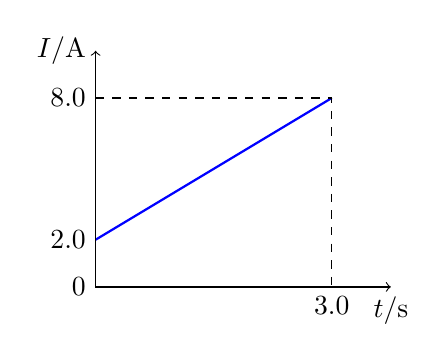
\begin{tikzpicture}[yscale=0.6]
		\draw[thick,blue] (0,1) -- (3,4);
		\draw[<->] (0,5) node[left]{$I$/A} -- (0,0) node[left]{0} -- (3.75,0) node[below]{$t$/s};
		\node[left] at (0,1) {2.0};
		\node[left] at (0,4) {8.0};
		\draw[dashed] (0,4) -- (3,4) -- (3,0) node[below] {3.0};
		\end{tikzpicture}
	\end{center}
	\vspace{-5pt}
\end{marginfigure}

\example{The current in a lamp is increased uniformly from 2.0 A to 8.0 A over 3.0 s. What is the charge flow?}

\begin{soln} Average current during this time is: $\bar{I} = \frac{2.0+8.0}{2} = 5.0 \text{ A} $

charge flow is then: $ Q = \bar{I} t = 5.0 \times 3.0 = 15 \text{ C} $

we can also use area under $I$-$t$ graph
\begin{equation*}
	Q = \frac{1}{2} \times (2.0 + 8.0) \times 3.0 = 15 \text{ C} 
\end{equation*}
\end{soln}

\subsection*{Microscopic view of electric currents}

The flow of electric current is essentially due to motion of charge carriers due to the electrostatic attraction and repulsion.\footnote{In most metallic conductors, charge carriers are those \emph{free electrons}. Charge carriers can also be thought about as positively-charged \emph{holes} (the absence of electrons) in some semi-conductors or \emph{ions} in chemical solutions.}
From an intuitive perspective, current would depend on number of charge carriers, and how fast they move. We'll see that this isn't far from correct. Let's take  a wire of cross section $A$, and see what follows in thinking about current.



\begin{figure}[ht]
	\centering
	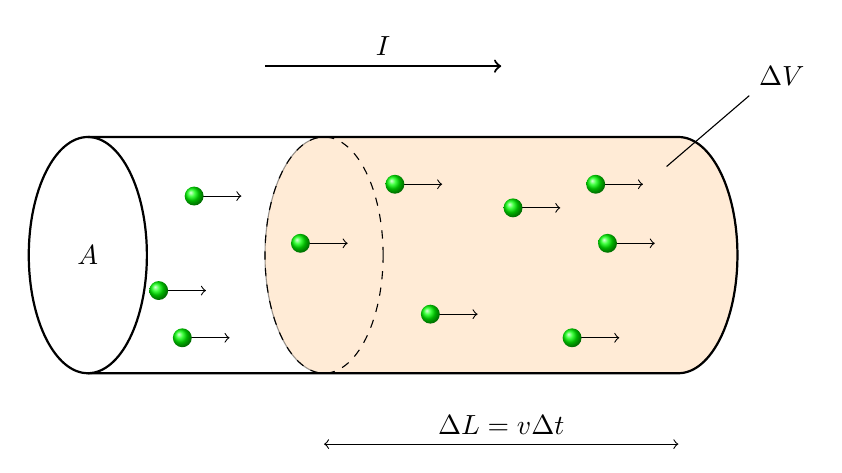
\begin{tikzpicture}[scale=1.5]
	\draw[fill=orange!40, opacity=0.4] (5,-1) arc(-90:90:0.5 and 1) -- (2,1) arc(90:270:0.5 and 1) -- (5,-1);
	\draw[thick] (0,0) ellipse (0.5 and 1) node {$A$};
	\draw[dashed] (2,0) ellipse (0.5 and 1);
	\draw[thick] (0,-1) -- (5,-1) arc(-90:90:0.5 and 1) -- (0,1);
	\foreach \x/\y in {0.6/-.3, 0.9/0.5, 0.8/-0.7, 1.8/0.1, 2.6/0.6, 2.9/-0.5, 3.6/0.4, 4.1/-0.7, 4.4/0.1, 4.3/0.6}{
	\draw[->] (\x, \y) --++ (0.4,0);% node[above]{$v$};
	\shade[ball color = green] (\x, \y) circle (0.08);
	}
	\draw[thick, ->] (1.5,1.6) -- (3.5, 1.6) node[midway, above] {$I$};
	\draw[<->] (2,-1.6) -- (5,-1.6) node[above, midway]{$\Delta L = v \Delta t$};
	\draw (4.9, 0.75) --++ (0.7,0.6) node[above right]{$\Delta V$};
	\end{tikzpicture}
\end{figure}



We know current is transfer of charge so let's define $n$ as the density of charge carriers for the material - in other words the number of charge carriers per unit volume: $n = \frac{\text{Number of free charges}}{\text{Volume}}$ 

The total number $N$ of charge carriers in a volume $V$ can then be given by: $N = nV$

If each carrier has a charge of $q$ and moves with a speed $v$, then they contribute to a current:
\begin{equation*}
	I = \frac{\Delta Q}{\Delta t} = \frac{\Delta N q}{\Delta t} = \frac{n \Delta V q}{\Delta t} = \frac{n A \Delta L q}{\Delta t} = \frac{n A v \Delta t q}{\Delta t} \RA \end{equation*} \begin{empheq}[box=\tcbhighmath]{equation*}{I = nAvq}
\end{empheq}

In metallic conductors, free electrons act as charge carriers, the equation becomes: $I = nAve$ where $e$ is the charge on an electron.

As with many statistical physics phenomena, the charge carriers have a distribution of speeds as they move 
so it's more proper to say that $v$ is actually an average velocity, called the \keypoint{mean drift velocity}

The charge density $n$ is a property of the material in question - ie it's value depends on type of material, good conductors have large $n$, while semiconductors have smaller $n$. \footnote{We're past the point of considering the world in binary terms of \emph{conductor} and \emph{insulator}, though we still use those terms as shorthand for the extremes of range.}


\example{A length of silver wire of a diameter of $1.2 \text{ mm}$ carries a current of 2.0 A. The electron number density in silver is $5.9\times10^{28} \text{ m}^{-3}$. What is the mean drift velocity of the electrons?}

\begin{soln}\begin{equation*}
v = \frac{I}{nAe} = \frac{I}{n\cdot\frac{1}{4} \pi d^2 \cdot e} \RA \end{equation*}
\begin{equation*}\frac{2.0}{5.9\times10^{28} \times \frac{1}{4}\pi \times (1.2\times10^{-3})^2\times1.60\times10^{-19}} \approx 1.9\times10^{-4} \mps
\end{equation*}

\eqyskip This calculation shows that each free electron actually travel at very low speeds in a wire \end{soln}

\example{A metal conductor and a piece of semi-conductor of the same cross section are connected in series. When an electric current is driven through them, compare the mean drift speed of the charge carriers in the two materials.}

\begin{soln}
    
The same current and same cross section, so mean drift speed $ v = \frac{I}{nAe} \propto \frac{1}{n}$

The metal has larger $n$, so free electrons move at relatively lower speeds

The semi-conductor has smaller $n$, so charge carriers move at relatively higher speeds \end{soln}




\subsection{P.d. \& e.m.f.}\label{ch:potential-difference}

Potential difference and e.m.f.\footnote{e.m.f. stands for \emph{electromotive force}, which is a miserably misleading term due to historical reasons. It has nothing to do with a force, or motivation for that matter. It is better to simply use the abbreviation e.m.f.} are both defined as the energy transfer per unit charge, both terms are often lumped together as \emph{voltages} in less formal contexts.

\begin{ilight}
	The \keypoint{P.d. (potential difference)} between two points is the energy converted from 
electrical potential energy to some other form per coulomb of charge flowing from one point to the other.: \begin{empheq}[box=\tcbhighmath]{equation*}{V=\frac{W}{Q}}\end{empheq} \index{potential difference}
\end{ilight}

\begin{ilight}
	\keypoint{The e.m.f. (electromotive force)} of a power supply is the energy converted from some other form (e.g. chemical) to electrical potential energy per coulomb of charge flowing through the source: \begin{empheq}[box=\tcbhighmath]{equation*}{\mathcal{E}=\frac{W}{Q}} \end{empheq}\index{e.m.f.}
\end{ilight}


The unit of measurement for p.d./e.m.f.: $[V] = [\mathcal{E}] = \text{V}$ (volt), where $1 \text{ V} = 1 \text{ J C}^{-1}$

The p.d. can tell you the direction of current flow through a component, current always flows from a higher potential to a lower potential.

We measure the p.d. across a component can be measured with a \keypoint{voltmeter}. 
\begin{marginfigure}
\centering
\begin{tikzpicture}[]
    \draw (0,0) to[rmeter,t=V] (2,0);
  \end{tikzpicture}
  \caption{The symbol for a Voltmeter}
\end{marginfigure}


\example{How much electrical energy is transformed into thermal energy when a charge of 10 C flows through a heater whose p.d. across is 25 V?}

\begin{soln}\begin{equation*}
	V = \frac{W}{Q} \RA W = V Q = 25 \times 10 = 250 \text{ J} 
\end{equation*}
\end{soln}
\example{A fully-charged 12 V car battery can supply a total electrical energy of 0.90 MJ. The starter motor of the car requires an average current of 150 A for a period of 2.0s. The battery is not able to recharge due to a fault. How many times can the starter motor be used?}

\begin{soln} total charge that can be supplied: $Q_\text{total} = \frac{W}{\mathcal{E}} = \frac{0.90 \times 10^6}{12} = 75000 \text{ C}$

charge needed for each start: $Q = I t = 150 \times 2.0 = 300 \text{ C}$

number of starts possible: $N = \frac{Q_\text{total}}{Q} = \frac{75000}{300} = 250$ \end{soln}

\example{Electrons beams are accelerated between a heated cathode and an anode with a potential difference of 40 V. What is the speed of the electrons when they reach the anode?}

\begin{soln} electrical potential energy is transformed into kinetic energy of electrons:
\begin{equation*}
qV = \frac{1}{2}mv^2 \RA 
\end{equation*}
\begin{equation*}
v=\sqrt{\frac{2qV}{m}} = \sqrt{\frac{2 \times 1.60 \times 10^{-19} \times 40}{9.11 \times 10^{-31}}} \approx 3.75 \times 10^6 \mps 
\end{equation*}
\end{soln}



\subsection{Resistance}

\begin{ilight}
	The \keypoint{Resistance}\index{resistance} $R$ of an electrical component is defined as the potential difference across divided by the current flowing through it: \begin{empheq}[box=\tcbhighmath]{equation*}{R=\frac{V}{I}} \end{empheq}
\end{ilight}


The unit of resistance: $ [R] = \text{V A}^{-1} = \Omega $ (ohm) named after Georg Ohm\footnote{Ohm's law was probably the most important of the early quantitative descriptions of the physics of electricity. We consider it almost obvious today. When Ohm first published his work, this was not the case; critics reacted to his treatment of the subject with hostility. They called his work a "web of naked fancies" and the Minister of Education proclaimed that "a professor who preached such heresies was unworthy to teach science." The prevailing scientific philosophy in Germany at the time asserted that experiments need not be performed to develop an understanding of nature because nature is so well ordered, and that scientific truths may be deduced through reasoning alone...}.

When a p.d. of 1 V is applied and current flow is 1 A, then resistance is 1 $\Omega$ 

Note that:
\begin{itemize}
    \item Resistance of a component does not depend on p.d. applied or current through it.
 \item Resistance $R$ of a component mainly depends on the following factors:

\begin{compactitem}
	\item[--] $R$ is proportional to length $L$ of the component: $R \propto L$.
	
	\item[--] $R$ is inversely proportional to cross-sectional area $A$ : $R \propto \frac{1}{A}$.
	
	\item[--] $R$ depends on the material of the component.
\end{compactitem}
\end{itemize}
this can be written as: \begin{empheq}[box=\tcbhighmath]{equation*}{R=\rho\frac{L}{A}} \end{empheq}

The constant $\rho$ is called the \keypoint{resistivity}\index{resistivity} of the material, a typical value of resistivity for a conducting metal is approx. $\rho \sim 10^{-8} \text{ } \Omega \text{ m}$.


\example{A current of 0.10 A is driven through a heater when connected to a supply voltage of 220 V. (a) Find the resistance of the heater. (b) If the heater is made from a wire of resistivity $1.8\times10^{-5} \text{ }\Omega\text{ m}$ and a diameter of 0.24 mm, find the length of the wire.}

\begin{soln}\begin{equation*}
	R = \frac{V}{I} = \frac{220}{0.10} \RA R = 2200 \text{ }\Omega
\end{equation*}
\vspace*{-1.2em}\begin{equation*}
R = \frac{\rho L}{A} \RA L = \frac{RA}{\rho} = \frac{2200 \times \pi \times (0.12\times10^{-3})^2}{1.8 \times 10^{-5}} \RA L \approx 5.5 \text{ m} 
\end{equation*}
\end{soln}
\example{A uniform wire of resistance $R$ has a length of $L$ and a cross-sectional area of $A$. If the wire is stretched to twice the length while its volume remains constant, what is the new resistance $R'$ in terms of $R$?}

\begin{soln}volume: $V=LA = \text{constant}$, so $A \propto \frac{1}{L}$, hence doubling $L$ means $A$ would become halved

\vspace*{0.3em} resistance: $R = \frac{\rho L}{A} \propto \frac{L}{A} \RA \frac{R'}{R}  = \frac{L'}{L} \times \frac{A}{A'} = 2 \times 2 \RA R' = 4R $ \end{soln}

\subsection{Electrical power}\index{power}

Current flowing through any electrical component causes energy to be transferred from source to the compnent. The rate at which electrical energy is transferred - the electrical power - is computed as:
\begin{equation*}
P = \frac{\Delta W}{\Delta  t} \xlongequal{V=\frac{W}{Q}} \frac{\Delta Q \cdot V}{\Delta t} \xLongrightarrow{I = \frac{\Delta Q}{\Delta t}} \end{equation*}
\begin{empheq}[box=\tcbhighmath]{equation*}{P=IV}
\end{empheq}

Substituting $V=IR$, the formula for electrical power also takes two useful forms:

\begin{empheq}[box=\tcbhighmath]{equation*}{P=I^2 R} \quad \text{or} \quad {P=\frac{V^2}{R}}
\end{empheq}

From these we can see why the national grid, and it's step-up and step-down transformers is such a big part of GCSE - You can see that a very small change in the current flowing can have a large impact on the power dissipated in the overhead wires. 

The unit of electrical power allows us to roll out a classic physics joke  \footnote{
\begin{tikzpicture}
\calloutquote[author=Teacher,width=3cm,position={(-1,-0.2)},fill=red!30,rounded corners]{What is the unit of power?}
\end{tikzpicture}
\begin{tikzpicture}
\calloutquote[author=Student,width=3cm,position={(1,-0.2)},fill=blue!30,rounded corners]{Watt!}
\end{tikzpicture}
\begin{tikzpicture}
\calloutquote[author=Teacher,width=3cm,position={(-1,-0.2)},fill=red!30,rounded corners]{Yes, What is the unit of power?}
\end{tikzpicture}} as it's the $Watt$. If a p.d. of 1 V drives a current of 1 A, power produced is 1 W, i.e., $1 \text{ W} = 1 \text{ A} \cdot 1 \text{ V}$



%\example{An electric toaster has a power rating of 900 W and current of 4.0 A. What is the resistance in the toaster?}
%
%\solc\begin{equation*}
%	P = I^2 R \RA R = \frac{P}{I^2} = \frac{900}{4.0^2} \RA R \approx 56 \text{ }\Omega 
%\end{equation*}



\example{An electric toaster is labelled `220 V 900 W'. When it is operating normally, find (a) the current through it, (b) the resistance in the toaster.}

\begin{soln}current: $I = \frac{P}{V} = \frac{900}{220} \RA I \approx 4.09 \text{ A}$

\vspace*{0.3em} resistance: $R = \frac{V}{I} = \frac{220}{4.09}$, $\,\,$ or alternatively, $R = \frac{V^2}{P} = \frac{220^2}{900} \RA R \approx 53.8 \text{ }\Omega$ \end{soln}

\example{Two conducting cylinders $X$ and $Y$ are of the same diameter and the same material. The length of the cylinder $X$ is twice of that of the cylinder $Y$. If the two cylinders are connected in series to a power supply so that the current through them are equal, find the ratio of the electrical powers dissipated in the two cylinders $\frac{P_X}{P_Y}$.}

\begin{soln} for either cylinder, electrical power: $P = I^2 R = I^2 \cdot \frac{\rho L}{A} = I^2 \cdot \frac{4 \rho L}{\pi d^2}$

same current $I$, same diameter $d$, same resistivity $\rho$, so power: $P \propto L \RA	\frac{P_X}{P_Y} = \frac{L_X}{L_Y} = 2 $ \end{soln}


\section{Electrical components \& $I$-$V$ characteristics}

Electrical circuits are all about the interplay of Voltage and Current. As such the key to understanding how different components behave differently when a p.d. is applied is through an $I$-$V$ characteristics graph.


\subsection{Ohmic conductors}

\begin{marginfigure}
	\centering
	\begin{tikzpicture}[scale=0.5]
	\draw[->] (0,-3) -- (0,3) node[left]{$I$};
	\draw[->] (-4,0) -- (4,0) node[below]{$V$};
	\draw[thick, blue] (-3.6,-2.7) -- (3.6, 2.7);
	\end{tikzpicture}
	
\end{marginfigure}

The resistance of an ohmic conductor is constant for all currents, so current is directly proportional to p.d.\index{Ohm's law}. Metal wires are usually considered as perfect ohmic conductors as the resistance of metal wires is nearly constant at fixed temperature. In a V-I graph, the resistance of an ohmic conductor equals the inverse of the gradient.



\subsection{Filament lamps}

\begin{marginfigure}
	
	\centering
	\begin{tikzpicture}[scale=0.5]
	\draw[->] (0,-3) -- (0,3) node[left]{$I$};
	\draw[->] (-4,0) -- (4,0) node[below]{$V$};
	\draw[thick, blue] (0,0) -- (1, 1.2) [out=50.2, in=190] to (3.6,2.7);
	\draw[thick, blue] (0,0) -- (-1, -1.2) [out=230.2, in=10] to (-3.6,-2.7);
	\end{tikzpicture}
	
\end{marginfigure}

Lamp filaments are usually made from tungsten because it has a very even emission across the visible range when how. It's also capable of sustained high temperatures (a fillament is essentially a demonstration of black-body radiation, which is why some bulbd tend to look yellow - they're not hot enough to be white). For small currents, the filament doesn't get hot enough to emitt light and behaves like an ohmic component. Larger currents cause the filaments to be heated to high temperature and the resistance to increase.\footnote{This is because the vibration of the metal lattice increases as the temperature goes up, free electrons are more likely to be scattered, so the metal becomes less conductive and the current does not increase as much for the same p.d. increase.}
To find resistance of lamp filament, we read off values of $I$ and $V$, then the ratio $\frac{V}{I}$  gives us the resistance.

\subsection{Thermistors}

\begin{marginfigure}
		\centering
	\begin{circuitikz}[european resistors]
		\draw[thick] (0,0) to [thR,l_=$R_T$] (3,0);
	\end{circuitikz}
\end{marginfigure}

A \keypoint{Thermistor}\index{thermistor} has a resistance that varies with temperature in a way you might not expect. As temperature rises, the resistance of the thermistor becomes lower\footnote{In A-Levels, we consider \emph{NTC (negative temperature coefficient)} thermistors only. This means their resistance decreases as temperature rises. \emph{PTC (positive temperature coefficient)} thermistors also exist but let's pretend they don't.}

The behaviour of thermistors can be explained in terms of band theory of solids. The material is behaving just like a wire, but there's an additional dominant effect: To put it in simple words, we can say that electrons are bound to atoms and cannot move freely at low temperatures, but they can gain energy and break free from atoms if temperature goes up. There are more free electrons available to conduct electricity, so resistance decreases. At greater currents, current increases more for same p.d. increase. 

\begin{figure*}[ht]
	\centering
	\begin{minipage}{0.55\textwidth}
		\centering
		\begin{tikzpicture}[scale=0.96]
		\draw[->] (-1.6,0) -- (5,0) node[below] {$T$/\OC};
		\draw[->] (0,0) node[below]{0} -- (0,4) node[right] {$R_T$};
		\draw[blue,thick] (-1.5,4) [out=-60,in=170] to (4.8,0.8);
		\end{tikzpicture}
	\end{minipage}\hfil
	\begin{minipage}{0.35\textwidth}
		\centering
		\begin{tikzpicture}[scale=0.6]
		\draw[->] (0,-3.2) -- (0,3.2) node[left]{$I$};
		\draw[->] (-3.5,0) -- (3.5,0) node[below]{$V$};
		\draw[thick, blue] (0,0) -- (1.2, 0.75) [out=32, in=250] to (2.8,3);
		\draw[thick, blue] (0,0) -- (-1.2, -0.75) [out=212, in=70] to (-2.8,-3);
		\end{tikzpicture}
	\end{minipage}
\end{figure*}

To find resistance of thermistor, we also compute the ratio $\frac{V}{I}$

\subsection{Diodes}

\begin{marginfigure}
	\vspace*{-5pt}
	\centering
	\begin{circuitikz}[european resistors]
		\draw[thick] (0,0) to [stroke diode,l_=$D$] (3,0);
	\end{circuitikz}
\vspace*{-16pt}
\end{marginfigure}

A \keypoint{diode} only allows current to pass in one direction\index{diode}. \cmt When an \emph{ideal} diode is forward-biased, $R_D \to 0$.

\cmt When an \emph{ideal} diode is reversed-biased, $R_D \to \infty$.

\begin{figure}[ht]
	\centering
	\begin{tikzpicture}[xscale=1.4, yscale=2]
	\draw[->] (0,-1.5) -- (0,3) node[left]{$I$};
	\draw[->] (-3.5,0) -- (5.2,0) node[below]{$V$};
	\draw[thick, blue] (-3.2,0) -- (1,0) node[below, black]{$V_\text{th}$} [out=0, in=268] to (2.1,3);
	\draw[<-] (2.15, 2) --++ (0.6, 0.2) node[right, note]{once $V>V_\text{th}$, diode has\\nearly zero resistance};
	\draw[<-] (0.4,-0.1) --++ (0.2,-0.6) node[below right, note]{if $V<V_\text{th}$, diode does not conduct};
	\draw[<-] (-1.5,0.1) --++ (-0.3,0.7) node[above, note]{diode has very high resistance\\when p.d. is reversed-biased};
	\end{tikzpicture}
\end{figure}

A practical semiconductor diode become conductive once p.d. reaches a set value $V_\text{th}$ called the diode's \emph{threshold voltage} (about $0.6\sim0.7$ V for a silicon diode). When a p.d. applied is forward-biased and greater than $V_\text{th}$, the diode has very low resistance, so there is a sharp increase in current once $V>V_\text{th}$

Though diodes have very high resistance if reversed-biased, if the reverse voltage reaches the \emph{breakdown voltage}, diode would become conductive\footnote{Typical breakdown voltage for a diode range from a few volts to several hundred volts, depending on its desired application.}





	
\subsection{End-of-chapter questions}

\question{
	A technician reports that the charge of an ion in a solution is measured to be $-5.5 \times 10^{-19} \text{ C}$. State and explain whether this measurement is reliable.
}


\question{
	Calculate the current that gives a charge flow of 300 C in one minute.
}

\question{
	The manufacturer of a car battery claims that the battery can supply a steady current of 40 A for one hour when fully-charged. (a) What is the charge flow through a point in the circuit in this time? (b) If a car requires a current of 90 A to start, for how long could the battery be used before recharging?
}

\question{
	A beam of $2.0 \times 10^{10}$ electrons travel through a distance of 0.50 m and are stopped on an electrode in a time period of $5.0 \times 10^{-8} \text{ s}$. (a) Find the charge collected on the electrode. (b) Find the average current produced by the electron beam.
}

\question{
	State the SI base units of number density $n$ and electric charge $q$, and hence show that the equation $ I = nAqv$ has consistent units on both sides.
}

\question{
	The number density of free electrons in copper is about $8.0\times10^{28} \text{ m}^{-3}$. If the current in a copper wire of diameter 0.50 mm is 0.80 A, calculate the average drift speed of electrons in the wire.
}

\question{
	Two coppers wires $A$ and $B$ are joined together and carry a current. If wire $A$ has diameter $d$ and wire $B$ has diameter $2d$, calculate the ratio of the average drift velocity of free electrons in the wires $\frac{v_A}{v_B}$
}

\question{
	From the calculations, we find that the drift speed of electrons in metal wires is around a few mm per second, so it would take a very long time for the free electrons to travel a distance of a few metres in an electric circuit. But when we switch on an electric lamp, it lights up immediately. Give a reason for this observation.
}


\question{
	When a p.d. of 15 V is applied across a wire of resistance 4000 $\Omega$, how many electrons would have passed a point in the wire in one minute?
}

\question{
	A motor has a resistance of 40 $\Omega$ and carries a current of 2.0 A. (a) What is the p.d. across? (b) At what rate is electrical energy being dissipated in the motor?
}


\question{
	A cable of 50 m is made of 19 parallel strands of copper wires. Each strand has a diameter of 0.25 mm. Given that the resistivity of copper is $1.7\times10^{-8} \text{ }\Omega \text{ m}$, find the resistance of the cable.
}


\question{
	A pencil is used to draw a line of length 20 cm, width 1.5 mm, and thickness 0.10 $\mu$m. The resistance of the line is 30 k$\Omega$. What is the resistivity of the material in the pencil?
}

\question{
	One resistor $P$ has a resistance of 16 $\Omega$. A second resistor $Q$ is made of the same material, but has twice the length but half the diameter. What is the resistance of $Q$? 
}

\question{
	A coil is made by wounding a long insulated wire of diameter $d$ onto a cylindrical core of diameter $D$ where $D \gg d$. If the coil has $N$ turns, and the resistivity of the wire is $\rho$, show that the resistance in the coil is $\frac{4N\rho D}{d^2}$.
}


\newpage



\question{
	If we want to determine the resistivity of the material of a length of metal wire, what measurements do we need to take?
}

\question{
	What is the current in a 40 W light bulb when a supply of 200 V is applied?
}

\question{
	Fuses of current ratings 1 A, 5 A, 10 A, 20 A are available. Suggest and explain which fuse should be used for a 120 V, 900 W hairdryer.
}

\question{
	A 12 V battery supplies a continuous current of 5.0 A for 3.0 hours. (a) Find the charge supplied by the battery during this time. (b) Find the energy produced from the battery.
}

\question{
	An electric cooker is labelled `240 V, 900 W'. (a) What is the resistance of the cooker's filament at its operating temperature? (b) State and explain whether there is any change in the resistance if it is measured at room temperature.
}

\begin{marginfigure}
	\vspace*{-18pt}
	\centering
	\begin{circuitikz}[european resistors]
		\draw (2,1.2) to[R, l_=$R$] (0,1.2) to[battery, l_=$\mathcal{E}$] (0,-1.2) -- (2,-1.2);
		\draw (2,1.2) to[stroke diode] (2,-1.2); 
		\draw (2,1.2) -- (4,1.2) to[rmeter, t=V] (4,-1.2) -- (2,-1.2);
	\end{circuitikz}
	\vspace*{-16pt}
\end{marginfigure}

\question{
	The diagram shows an electric circuit incorporating a diode, connected in series with a 5.0 $\Omega$ resistor across a battery having an e.m.f. of 3.0 V. If the diode and the voltmeter are both ideal, suggest the reading on the voltmeter (a) for the circuit shown, (b) if the diode is reversed.
}



\begin{marginfigure}
	\vspace*{-8pt}
	\centering
	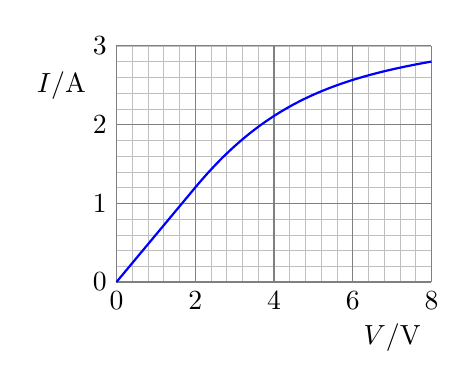
\begin{tikzpicture}
	\draw[very thin, gray!50, step=0.2] (0,0) grid (4,3);
	\draw[gray, step=1] (0,0) grid (4,3);
	\draw[thick, blue] (0,0) -- (1, 1.2) [out=50.2, in=190] to (4,2.8);
	\foreach \I in {0,1,2,3} \node[left] at (0,\I) {$\I$};
	\foreach \V in {0,2,4,6,8} \node[below] at (\V/2, 0) {$\V$};
	\node at (3.5, -0.7) {$V$/V};
	\node at (-0.7, 2.5) {$I$/A};
	\end{tikzpicture}
	\vspace*{-16pt}
\end{marginfigure}

\question{
	The diagram shows the $I$-$V$ characteristics of an electrical component $P$. (a) Suggest whether $P$ a filament lamp or a thermistor. (b) What is the resistance of $P$ for a current of 2.8 A? (c) Draw on the same graph the $I$-$V$ characteristics for a fixed resistor $Q$ of 4.0 $\Omega$. (d) Compare the power dissipated in $P$ and $Q$ for a p.d. of 4.0 V.
}







